\section{Direct orbit trasnfers}

This section presents the results computed for a direct orbit transfer between
Earth and the two interstellar objects. The analysis is performed by solving the
Lambert's problem under the Keplerian assumption. In addition, the modulus of
the escape velocity for Earth, $\Delta_e = 11.20$ km/s, is added to the required
launch velocity, leading to more realistic values.

The algorithm used is the one presented by \cite{izzo2015}, as it is proven to
be more accurate and faster than other classical algorithms \cite{martinez2021}.
The ephemerides for 'Omuaumua and 2I/Borisov are obtained from JPL Horizons API
service at epoch January 1, 2018. These are propagated under the two-body
assumption to simplify the analysis. Maximum propagation date is January 1,
2035.

Porkchop plots for 'Oumuaumua and 2I/Borisov are shown in figure
\ref{fig:oumuamua-direct-transfer-porkchop} and figure
\ref{fig:borisov-direct-transfer-porkchop}. The limits for the characteristic
energy range between 0 and 12000 km$^2$/s$^2$.

\begin{figure}[H]
  \centering
  \includegraphics[width=\textwidth]{static/oumuamua/direct-transfer-porkchop.png}
  \caption{Launch energy porkchop plot for 1I/'Oumuamua.}
  \label{fig:oumuamua-direct-transfer-porkchop}
\end{figure}
\begin{figure}[H]
  \centering
  \includegraphics[width=\textwidth]{static/borisov/direct-transfer-porkchop.png}
  \caption{Launch energy porkchop plot for 2I/Borisov.}
  \label{fig:borisov-direct-transfer-porkchop}
\end{figure}

The contour maps show a periodic pattern, with a minimum energy transfer
corridor every year. This year corresponds to a more favorable position of the
Earth with respect to the interstellar object.

The most energy consuming area is located in the lower right corner of the plot.
This area corresponds to a shorter time of flight (4 years). The shorter the time of
flight, the greater the launch velocity and the energy required to perform the
transfer. On the other hand, the upper left corner corresponds to a longer time
of flight (17 years), with lower energy requirements.

It is worh noting that the energy required to reach 1I/'Oumuamua is slightly lower
than the energy required to reach 2I/Borisov. This is due to the higher velocity of
this object, since 1I/'Oumuamua is travelling at $26.0$ km/s whereas 2I/Borisov does
at $32.2$ km/s.

Finally, both porkchops show a similar contour map. This is due to the long
distance exhibited by the two interlopers in the future positions depicted in
the porkchop plot. The short-time transfer scenarios show differences between
'Oumuamua and 2I/Borisov, but the long-time transfer scenarios show close values.

\begin{figure}[H]
  \centering
  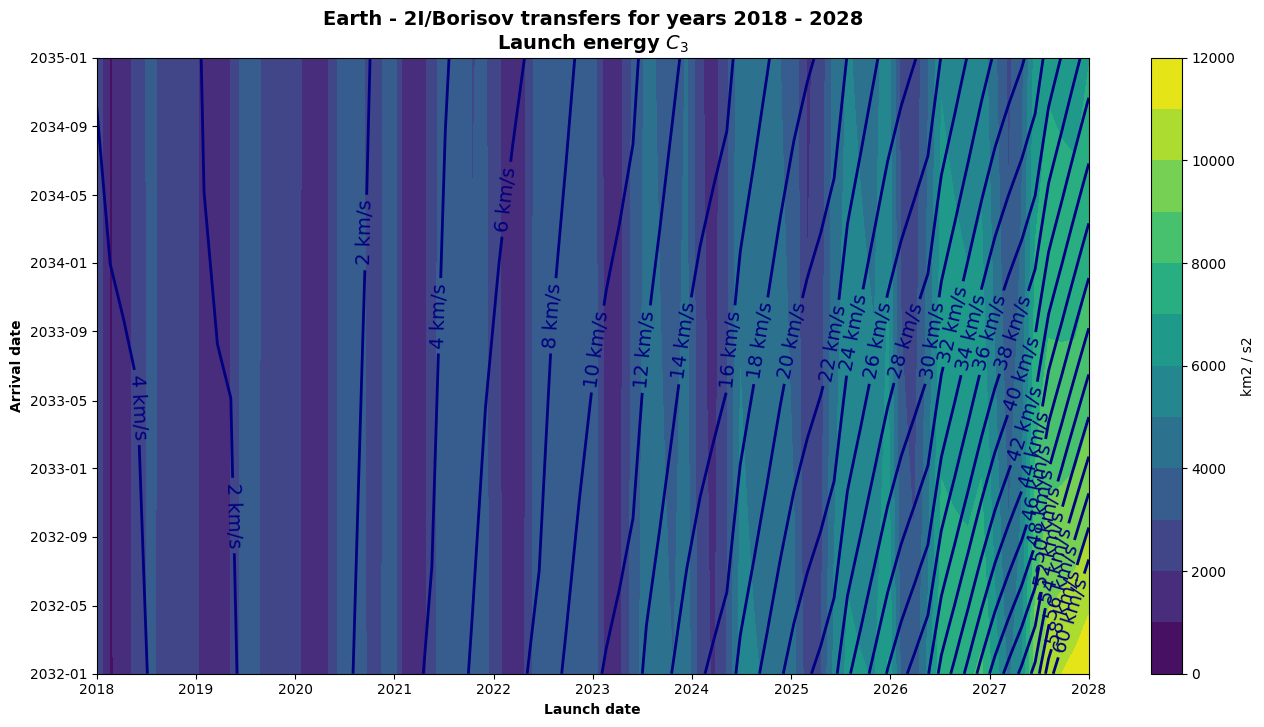
\includegraphics[width=\textwidth]{static/borisov/direct-transfer-porkchop-avl.png}
  \caption{Launch energy porkchop plot for 2I/Borisov.}
  \label{fig:oumuamua-direct-transfer-porkchop}
  \label{fig:borisov-direct-transfer-porkchop-avl}
\end{figure}


